\documentclass[conference]{IEEEtran}
\IEEEoverridecommandlockouts
% The preceding line is only needed to identify funding in the first footnote. If that is unneeded, please comment it out.
\usepackage{cite}
\usepackage{amsmath,amssymb,amsfonts}
\usepackage{algorithmic}
\usepackage{graphicx}
\usepackage{textcomp}
\usepackage{xcolor}
\def\BibTeX{{\rm B\kern-.05em{\sc i\kern-.025em b}\kern-.08em
    T\kern-.1667em\lower.7ex\hbox{E}\kern-.125emX}}



\begin{document}

\title{
    Securing Windows Subsystem for Linux \\
    A Behavioral Detection Approach
}
% {\footnotesize \textsuperscript{*}Note: Sub-titles are not captured in Xplore and
% should not be used}
% \thanks{Identify applicable funding agency here. If none, delete this.}
% 

\author{
    \IEEEauthorblockN{1\textsuperscript{st} Andrei Mermeze}
    \IEEEauthorblockA{
        \textit{dept. name of organization (of Aff.)} \\
        \textit{name of organization (of Aff.)} \\
        Cluj-Napoca, Romania \\
        andrei.mermeze@gmail.com
    }
\and
\IEEEauthorblockN{2\textsuperscript{nd} Phd. Radu Dragos}
\IEEEauthorblockA{\textit{dept. name of organization (of Aff.)} \\
\textit{name of organization (of Aff.)}\\
City, Country \\
email address}
}

\maketitle

\begin{abstract}
The release of Windows Subsystem for Linux (WSL) revealed a whole new attack surface, comprised of kernel drivers as well as user-mode services.
The performed research is going to reveal how behavioral detection techniques can be applied for detecting potential threats (bashware) that abuse WSL.
This paper will provide an insight into the security issues created by this subsystem, while also explore both Kernel-Mode and User-Mode based
detection heuristics and techniques in order to identify and block this new type of malware. First sections focus on WSL internals, whereas the
next sections present what mechanisms can be used to acquire the needed information for identifying bashware, and finally some heuristic
behavioural based approaches on identifying the bashware.
\end{abstract}

\begin{IEEEkeywords}
Windows Subsystem for Linux Security Behavioral Analysis Malware Bashware Detection Event Tracing Minifilter Monitoring Kernel Driver
\end{IEEEkeywords}

\section{Introduction}
Windows Subsystem for Linux was first released in the annniversary update and it provides a way of executing Linux ELF 64 bit binaries on
native Windows 10. Since WSL is not a virtualization based system, the Linux processes running in it can access any resource on the computer,
making it a dangerous threat until a AV Solutions are updated to support this new type of processes.\\

\section{Overview of WSL}
 
    \subsection{Minimal Processes and Pico Processes}
    A minimal process has a parent, protection level, name and security token. It has no initial thread, no process enviroment-block (PEB),
    no ntdll, and its address space is empty. Its threads are called "minimal threads", and, similarly to minimal processes, they have no
    thread enviroment block (TEB). A pico process is a minimal process, but it has an associated pico provider, which handles the system calls,
    exceptions, pico process or threads creation and termination.\\

\subsection{Pico Providers}
    A pico provider is a kernel driver that implements the required functionalities to handle pico process events. Registering as a pico provider
    is done by calling the PsRegisterPicoProvider API, however, calling this API requires that the PspPicoRegistrationDisabled is set to FALSE.
    This value is set to false before any other third party driver is loaded, therefore, at least for now, it is not possible to implement
    custom pico providers. In order to secure pico providers, they also register with PathGuard in order to protect its syscalls. Kernel Patch
    Protection, also known as PatchGuard, was designed to protect kernel structures from being patched. This renders the classic linux
    monitoring solution (syscall hooking) useless, as any attempt to hook the syscalls will result in a BSOD (Blue Screen of Death).\\

    \par{}
    Lxcore.sys does the pico provider registration in the LxInitialize function, which is called by lxss.sys in its DriverEntry.
    \begin{figure}[htbp]
        \centerline{
\includegraphics{PsRegisterPicoProcess.png}}
        \caption{lxcore.sys pico provider registration}
        \label{fig1}
    \end{figure}

\subsection{Sycalls}

    Currently, as of Windows 10 1709, 242 Linux syscalls are implemented in lxcore.sys. These syscalls are implemented as callbacks that reside
    in a table (lxcore!LxpSyscalls), and are called from lxcore's LxpSysDispatch callback, which was registered with PsRegisterPicoProvider.\\

\subsection{File System}

\begin{itemize}
    \item VFS
    \item VolFs - /mnt/c
    \item DrvFs - /drv
    \item SysFs - /sys
    \item TmpFs - /tmp 
    \item ProcFs - /proc
\end{itemize}



\section{Exploring the Attack Surface}
    Lxcore is the core kernel-mode component of WSL that implements the Linux syscalls, multiple filesystems, and all the logic for running
    linux binaries in Windows. The driver, being responsible with providing the kernel support for user processes, implements many parsing
    algorithms (i.e. ELF header parsing, user strings parsing), making it prone to overflows, off-by-ones and many other issues that can be
    used in developing exploits, as we will see in the next section.\\

\section{Known Vulnerabilities}

    \subsection{Execve Exploit}
    Was discovered by Saar Amar, and was given the following CVE: CVE-2018-0743. The exploit leverages an integer overflow in
    lxcore!LxpUtilReadUserStringSet in order to run privilleged code. The shellcode elevates a process given by its pid. In this paper we are going
    to explain in detail the algorithm we came up with.\\

    \subsection{Local Denial of Service}
    While experimenting with Event Tracing for Windows and reversing lxcore, we've discovered an issue in lxcore allowing us to trigger a
    BSOD from an unprivilleged user-mode process. However, due to responsability disclosure, we will not go into any more
    detail about this issue until it is patched by Microsoft.\\

\section{Monitoring WSL Activity}

    There are multiple ways of monitoring WSL activity, which, if correctly combined, can provide enough information in order to identify
    potentially malicious activity.\\

    \begin{itemize}
        \item User-Mode Hooking Framework - API usage monitoring
        \item File System Minifilter - file system I/O and process monitoring
        \item Event Tracing for Windows
        \item Windows Filtering Platform - network monitoring    
    \end{itemize}

    \par{}
    While we've studied and experimented with all of the above, we focused only on the file system minifilter approach, therefore we won't go into
    great detail about the other methods.\\

\subsection{User-Mode hooking driven WSL monitoring}
    
    In order to obtain more granular monitoring capabilities, a function hooking framework is required. The ability of synchronously monitoring
    specific API usage opens up a range of possibilities, from exploit detection to syscall graph based detection heuristics.
    In order to load a shared library into any Linux pico process, an entry with the path to the library must be added into the ld.so.conf. Since
    any process with root privilleges (inside the linux system) can update the said config file, we must protect it from a kernel driver, so that
    we are sure that our shared library isn't removed. This can be done by filtering IRP\textunderscore MJ\textunderscore WRITE operations on that
    file and readding the entry if removed.\\
    
    \par{}
    When loaded in a linux process, the library hooks the functions we want to monitor (i.e. ptrace, open) and synchronously notifies a 
    service via local sockets about every hooked function call, informing the service about exploitation intent and failing the function call
    if needed.\\

    \par{}
    We consider this method unreliable against smarter bashware that actively checks and avoids hooked functions, and possibly completely useless
    starting with Windows RS5 if executable memory can't be allocated anymore.\\

    % \subsection{ETW driven WSL monitoring}

    % Lxcore is traced using ETW TraceLogging APIs, thus providing a way of monitoring WSL activity from a user-mode Windows process.\\
    % \subsubsection{ETW}


    % \subsubsection{Leveraging ETW in WSL activity monitoring}
    % Lxcore registers two event providers.\\
    % Microsoft.Windows.Lxcore logs informative events, such as process or thread creation and termination as well as events that might indicate
    % malicious intent, for example syscall fuzzing by trying to call unimplemented syscalls.\\

\subsection{Using A File System Minifilter to Monitor WSL Activity}
    
    This is the most reliable way of monitoring and blocking potentially malicious Linux applications. Unlike a user-mode hooking framework
    approach, using a Windows driver provides mechanisms of monitoring that cannot be bypassed or tampered with by the monitored processes, making
    it a very reliable and secure approach.\\

    \par{}
    The driver we've implemented filters file system I/O and also keeps track of active processes. In the next sections we are going to present
    how we implemented the driver.\\
    
    \subsubsection{File System Filtering}
    In Windows I/O request packets(IRPs) are used to communicate between drivers. For example, in the context of the file system, IRPs are used
    to describe file I/O operations, like file read (IRP\textunderscore MJ\textunderscore READ) or file create
    (IRP\textunderscore MJ\textunderscore CREATE). A minifilter driver can register pre and post callbacks for all IRPs by
    calling FltRegisterFilter. As the name suggests, the pre callback is called before the operation is completed and the post callback is
    called after the operation is completed. For example, the pre callback for an IRP\textunderscore MJ\textunderscore CREATE would show the intent
    of creating or opening a file, but only in the post callback we would know if it succeeded or not (file might not exist in case of an open).\\

    \par{}
    We've used this technology in order to monitor linux processes as well as win32 processes file system activity. We have decided to only monitor
    win32 processes that are part of a linux process tree (an ancestor of the process is a linux process) in order to reduce the performance
    overhead.

    \par{}
    When filtering, we are mostly interested in 2 fields of the FLT\textunderscore CALLBACK\textunderscore DATA structure, while the
    FILE\textunderscore OBJECT is taken from the FLT\textunderscore RELATED\textunderscore OBJECTS structure.\\

    \begin{verbatim}
0: kd> dt fltmgr!_FLT_CALLBACK_DATA
...
0x10 Iopb         : Ptr64 _FLT_IO_PARAMETER_BLOCK
...
0x50 RequestorMode: Char

0: kd> dt fltmgr!_FLT_RELATED_OBJECTS
...
0x20 FileObject   : Ptr64 _FILE_OBJECT
...

    \end{verbatim}
    Iopb field, containing the operation's parameters (i.e. share access for IRP\textunderscore MJ\textunderscore CREATE or Length for
    IRP\textunderscore MJ\textunderscore READ) and the RequestorMode field, which tells us if the IRP was issued by the kernel or not.\\

    \par{}
    The main difference between filtering I/O requests issued by win32 processes and Linux processes is that, for Linux processes,
    the RequestorMode is KernelMode, because IRPs are issued by the kernel, not by the actual process. That is because linux processes don't know
    of Windows IRPs, therefore the pico provider has to translate the I/O request into an IRP. Considering this, we filtered kernel
    issued IRPs too, but only those for which the requestor id was not system's PID. To do this, in the pre callback for every irp we checked
    PFLT\textunderscore CALLBACK\textunderscore DATA RequestorMode field, and if the requestor pid returned by FltGetRequestorProcessId is 4
    (system process pid) or if the pid was of a win32 process that is not part of linux process tree, then we return
    FLT\textunderscore PREOP\textunderscore SUCCESS\textunderscore NO\textunderscore CALLBACK, thus skipping an unecessary call to the
    post callback.\\


    \subsubsection{Process Filtering}
    In order to receive process creation and termination notifications, the driver must register a callback with
    PsSetCreateProcessNotifyRoutineEx2. This callback will be called synchronously for both win32 processes and pico processes. The algorithm
    on process creation is as follows:
    \begin{itemize}
        \item get the process' initial security token and check for initial privillege escalation
        \item determine if it is a WSL process
        \item insert the process in the process collector if it is a WSL process or if parent is in the collelctor
        \item insert the process in its parent process tree if it exists, else create a new process tree
    \end{itemize}
    
    \par{}
    Before any other processing is done, we need to check for a potential privillege escalation at process startup. We do this by checking if
    the process was elevated in any other way except by svchost or by an already elevated parent. Process elevation will be detailed in the
    privillege escalation detection section.\\

    \par{}
    In order to identify a WSL process, the driver must call ZwQueryInformationProcess with SubsystemInformationTypeWSL information type on the
    process' handle and check that the subsystem type is SubsystemInformationTypeWSL (linux process) or SubsystemInformationTypeWin32
    (win32 process). After determining the subsystem we insert an entry into our process collector if the subsystem type is
    SubsystemInformationTypeWSL or if it's parent is already in the collector. This way we are sure that we monitor win32 processes too, if and
    only if they are part of a linux process tree. If its parent is already in the collector, we add it as a child process in its tree, else we
    create a new process tree.\\

\section{Detection Heuristics}
    \subsection{Ransomware}
    Ransomware is a type of malware that encrypts the users' files and demands money, usually in the form of crypto currency, like bitcoin,
    in order for the user to regain access to the files. More advanced ransomware could go as far as preventing the operating system to boot
    until the payment is made. An example of such ransomware would be petya.\\

    \par{}
    A ransomware that targets WSL would be leverage the fact that most AV minifilters do not filter IRPs that are coming from the kernel, allowing
    the ransomware to silently encrypt files. Even more, the ransomware might silently communicate with a server without being detected by network
    filters.\\

    \par{}
    A reliable solution would be to monitor kernel issued IRPs that are done on behalf of a Linux process, and to use a either a scoring engine
    or some AI expert system (i.e. Support Vector Machine) to identify the ransomware. We are going to cover only the behavioral heuristics
    approach in this paper.\\

    \par{}
    In case of a scoring engine, the process could be assigned points according to the file system activity it does. For example, a file
    delete or write would add more points than a file read. Moreover, even more points could be added if the action involves sensitive paths
    (i.e. system root, Windows directory, etc). When the process reaches a certain threshold, a detection alert should be issued and the process
    should be killed. In order to detect multi-process ransomware we keep track of its whole process tree.\\

    \par{}
    In order to do this, we keep a dictionary (internally, a trie) with all paths we monitor. Each path has an associated score for each I/O
    operation. The operations we are mostly interested in are file move, extension change, file delete, file write, file create. The score we
    keep per path per operation is heuristiclaly chosen and can be fine tuned using different machine learning algorithms. Whenever an operation
    is filtered, we try to match the path against our dictionary, and add the coresponding points if the path was matched.\\

    \par{}
    Matching paths for each file operation can be a costly operation. We had to come with a caching mechanism so that when we matched a path,
    we would known the scores we need to assign for any operation without rematching the path. We've decided that the best solution was using
    file contexts. The minifilter driver defines the context's structure and assigns it to a filter manager object(i.e. volume, file, stream handle,
    etc). In our case, the context is a structure that contains the array of scores for the monitored operations. This way, whenever we filter a
    file operation, we check if it has a context associated with it (FltGetFileContext). If a context already exists, then we just add points for that process. If not,
    we allocate (FltAllocateContext) and set the context (FltSetFileContext), then add the points.

    % \par{}
    % We could further improve the algorithm by adding an exception mechanism, in order to allow certain operations for known fewer points to processes that are known to access certain Windows paths,
    % for example, a latex compiler that writes the compiled PDF in the user's "Documents" folder. 

    \subsection{Windows Privillege Escalation}
    Privillege escalation is a powerful exploit that is meant to elevate an unelevated process without users' consent or knowledge. It is very
    important to understand the elevation process in order to identify the exploit. In this section we are going to describe in detail how
    elevation is done in Windows and how we can detect the exploit.\\

    \par{}
    On Windows, there are multiple ways of starting an elevated process:
    \begin{itemize}
        \item from an unprivileged process, via ShellExecuteEx % through UAC (User Account Control)
        \item auto elevate via manifest
        \item from a privileged process
    \end{itemize}

    \par{}
    When an unprivileged process needs to start a privileged process, it sends a request to svchost, which shows the User Account Control pop-up
    through consent.exe, notifying the user that the process needs admin rights. If admin rights are granted by UAC, svchost starts the process.
    If a process already is elevated, any process spawned by it will also be elevated. We can easily see that, if wsl.exe is started with admin
    rights, all Linux processes running in that WSL instance will be granted admin rights inside Windows, which would be disastrous considering
    the security of the machine.\\
    
    \par{}
    This kind of exploit can be detected easily, while not very reliable, from a kernel driver, or, more reliable, by using memory introspection
    techniques from a hypervisor. While the latter is extremly reliable, it is much more complex than a kernel-driver. We will cover only the
    first technique and try to make it as reliable as possible without adding too much performance overhead.\\
    
    \par{}
    We need to check that the process' token was not tampered with. The algorithm for checking if a process is elevated is fairly simple. We use
    ZwOpenProcessTokenEx to get the process' security token and then ZwQueryInformationToken with TokenElevation information class. The
    returned boolean will tell if the process is elevated or not. This check can easily be done at in the process notification callback because
    we get the process' handle as a parameter.\\
    
    \par{}
    Seeing how execve exploit works, it is clearly obvious that while this method works for the most basic case, it is quite unreliable.
    That's becausewe need to  poll the security token at certain moments since the exploit just overwrites the process' security token with
    the System security token. Such key moments would be whenever we intercept actions that would naturally require admin privilleges,
    i.e. acessing the Windows or System32 folders.
    It's easy to see several issues:\\

    \begin{itemize}
        \item if the exploit elevates the current process while running
        \item if the exploit is used to elevate another process
        \item if the elevated process is a Windows process
        \item performance overhead added by polling the security token
    \end{itemize}

    Further, we are going to explain how we've tackled these problems and made the algorithm more reliable.\\

    \subsubsection{Detecting privillege escalation on already running processes}
    In order to do this we need to keep track of all active processes in a structure that we'll call a process collector. When we add a new process
    into the collector, we will also store its initial elevation. Then, whenever the processes does sensitive actions, like dropping executables
    in paths like "C:\textbackslash Windows", we will recheck the security token with the algorithm previously presented. If the new elevation differs from the
    initial elevation, the process should be detected and killed.\\

    \subsubsection{Detecting elevation of a running Windows process}
    We applied the same algorithm for Windows processes that are started by Linux processes as well, with two observations:
    We need to keep track of Windows processes as well, but only if they are part of a process tree that has a Linux process as well, and we
    need to detect and kill the whole process tree.\\

    \begin{figure}[tb]
        \centering
        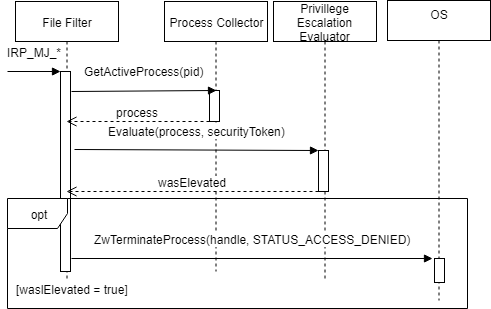
\includegraphics[width=\columnwidth]{DetectionDiagram.png}
        \caption{privillege escalation detection diagram}
        \label{fig2}
    \end{figure}

    \subsubsection{Minimizing the performance overhead}
    Polling the security token for every Linux process would become costly performance-wise very quickly, if the process does I/O
    intensive operations(i.e, a compiler). It is neccessary to narrow the set of actions for which we do security token registraiton, as well
    as use an efficient algorithm for matching strings against a predefined dictionary.\\


\begin{thebibliography}{00}
\bibitem{b1} Pavel Yosifovich, Alex Ionescu, Mark E. Russinovich, and  David A. Solomon ``Windows Internals''
\bibitem{b2} Alex Ionescu ``THE LINUX KERNEL HIDDEN INSIDE Windows 10,'' BlackHat2016
\bibitem{b3} Alex Ionescu ``GAINING VISIBILITY INTO LINUX BINARIES ON Windows: DEFEND AND UNDERSTAND WSL,'' BlueHat2016
\bibitem{b4} Saar Amar ``LINUX VULNERABILITIES, Windows EXPLOITS Escalating Privileges with WSL,'' BlueHat2018
\bibitem{b5} Manuel Egele, Theodoor Scholte, Engin Kirda, and Christopher Kruegel ``A Survey on Automated Dynamic Malware Analysis Techniques and Tools,'', ACM Computing Surveys (CSUR) ,February 2012
\end{thebibliography}
\end{document}
